\section{Experimental Results}
\label{Experimental Results}

\subsection{Simulation Environment}
\begin{figure}[h] 
    \centering
  \subfloat[]{%
       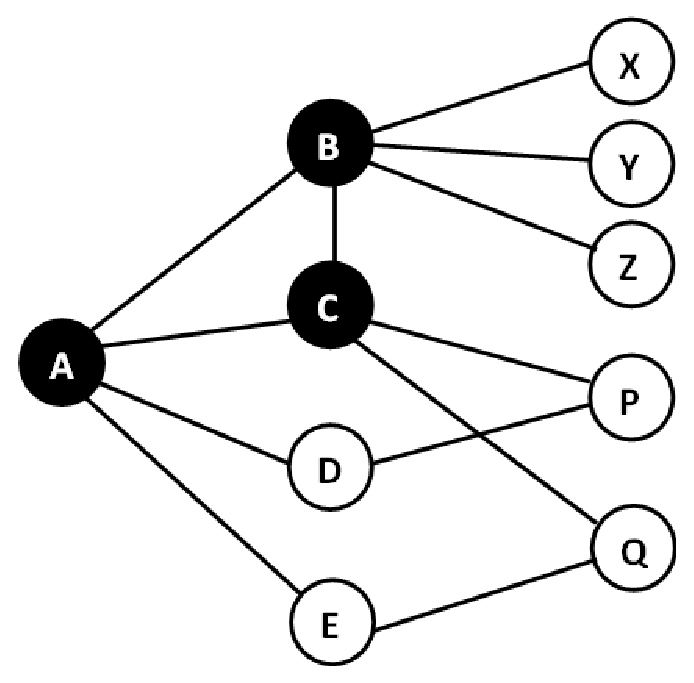
\includegraphics[width=0.45\linewidth, height=35mm]{Figures/forwarding1.eps}}
    \label{subfig1}\hfill
  \subfloat[]{%
        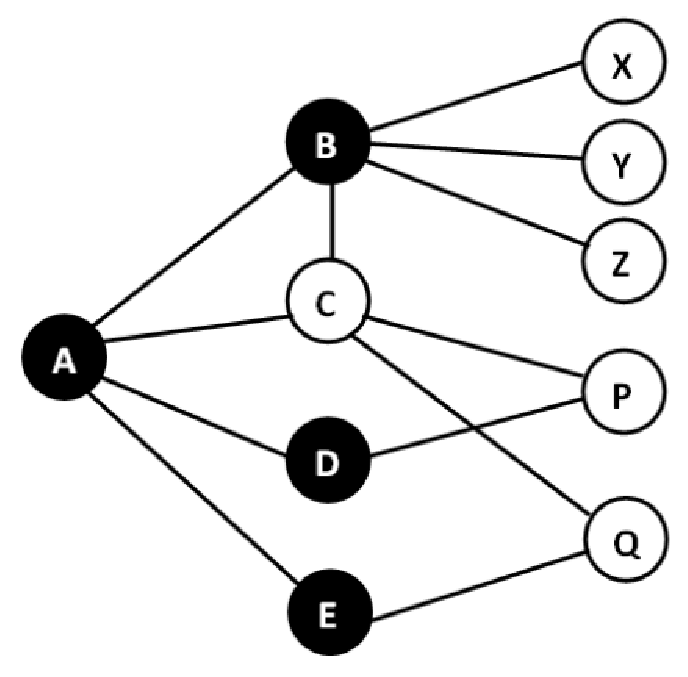
\includegraphics[width=0.45\linewidth, height = 35mm]{Figures/forwarding2.eps}}
    \label{subfig2}\\
  \caption{(a) CDS to minimize redundancy, (b) CACDS to minimize contention}
  \label{ac} 
\end{figure}
To evaluate the performance, randomly deployed networks of 100-500 nodes over a fixed 625m X 625m square region has been simulated. The transmission radius is limited between 125m to 225m. 
%Each node is placed randomly in the simulation space for testing purpose. 
For each scenario 10 different networks are generated and the mean value of the number of forwarding nodes and the amount of contention are taken to evaluate the effectiveness of the proposed algorithms. The simulation code-base is built using C++ programming language. 

\subsection{Performance Metrics}
While evaluating the algorithms, the number of forwarding nodes and the number of contention have been chosen as performance metrics.
%\begin{enumerate}

 \textbf{ (i) Number of forwarding nodes:} The total number of forwarding nodes needed to complete a broadcast is same  as the size of a CDS. Thus we calculate the size of the constructed CDS to determine number of forwarding. In order to minimize contention, the nodes that can reach the maximum number of nodes in the network may to get selected. Therefore, the number of forwarding nodes might increase in order to mitigate contention.  Such a scenario is depicted in Figure \ref{ac}. The number of forwarding nodes is 3 in traditional MCDS algorithm. The number of forwarding nodes increases to 4 in order to minimize contention.

  \textbf{ (ii) Number of Contention:} The total number of contention to complete a broadcast is determined as follows. At first we define ``per hop contention'' which is the number of nodes in the forwarding list of any node $v$ that are neighbors of each other. If one of the members of the $F\textsubscript{v}$ is connected (within the transmission range) to another ones, then those nodes face contentions when they try to forward the packet. Thus per hop contention  ($\mathcal{P}$) is mathematically determined as:  
  $$  \mathcal{P}(v) = \sum_{w \in F\textsubscript{v}} \Big(\big|(N(w)-\{w\}) \cap F\textsubscript{v}\big|\Big)/2$$
Suppose, to complete a broadcast the nodes in $\mathcal{S} = \{v_1,v_2,v_3, ... , v_{cacds}\}$ forward the packet, i.e., $\mathcal{S}$ is the CDS. Let $\mathcal{F}$ represents the set of all the forwarding list that are created at each hop. $$\mathcal{F} =  \{F_{v_1},F_{v_2},F_{v_3},....,F_{v_{cacds}} \}$$
 When we sum up per hop contention of all the forwarding nodes in the network, we get the total number of contention $\mathcal{N}$ that would occur for a broadcast which is mathematically defined as: 
$$  \mathcal{N} = \sum_{v_i \in \mathcal{S}} \mathcal{P}(v_i)= \sum_{v_i \in \mathcal{S}} \sum_{w \in \mathcal{F}_{v_i}}\Big(\big|(N(w)-\{w\}) \cap \mathcal{F}_{v_i}\big|\Big)/2 $$

%\end{enumerate}
\subsection{Experimental Results regarding Number of Forwarding}
For better readability of the results, we have separated the graphs of centralized (MCDS and Centralized CACDS) and distributed (DP and distributed CACDS) algorithms. In Figure \ref{outf100c} and \ref{outf100d}, the effect of centralized and distributed algorithms is presented. The number of node has been set to 100. The size of Centralized CACDS and MCDS is almost same for this scenario. In distributed environment, proposed algorithm needs 1-5\% additional transmissions which is not very high. 
 \begin{figure}[h]
    \centering
    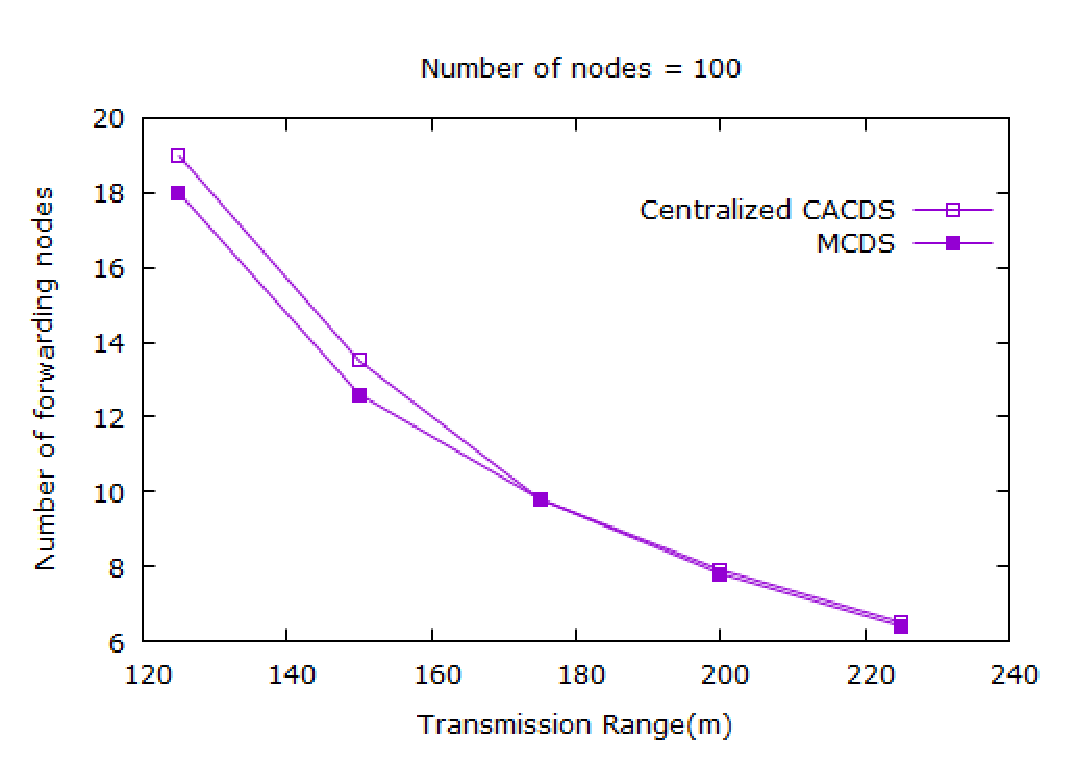
\includegraphics[width=90mm, height=57mm]{Figures/outf100c.eps}
    \caption{Performance of Centralized Algorithms for number of required transmissions of networks having 100 nodes by varying transmission range}
    \label{outf100c}
    \end{figure}
    
    \begin{figure}[h]
    \centering
    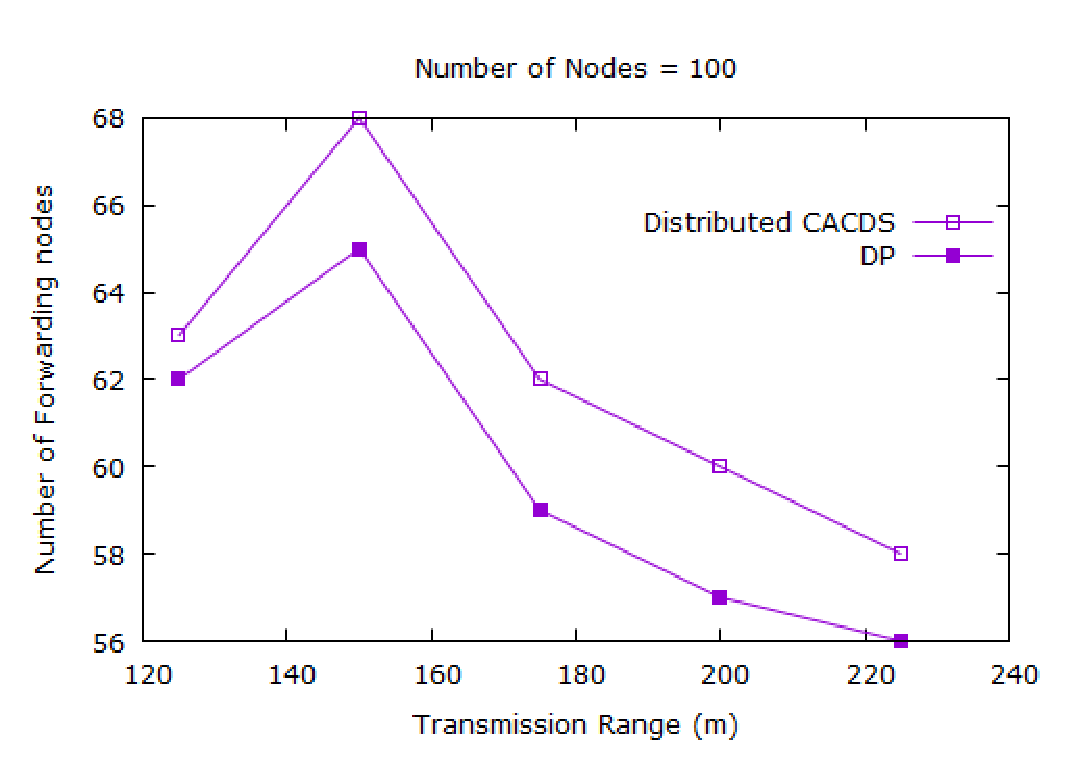
\includegraphics[width=90mm, height=57mm]{Figures/outf100d.eps}
    \caption{Performance of Distributed Algorithms for number of required transmissions of networks having 100 nodes by varying transmission range}
    \label{outf100d}
\end{figure}

Figure \ref{outf225c} and \ref{outf225d} shows the required transmissions by adding nodes in a fixed transmission range (225m). Here also the difference in number of forwarding nodes is very small for both centralized and distributed cases. 
\begin{figure}[h]
    \centering
    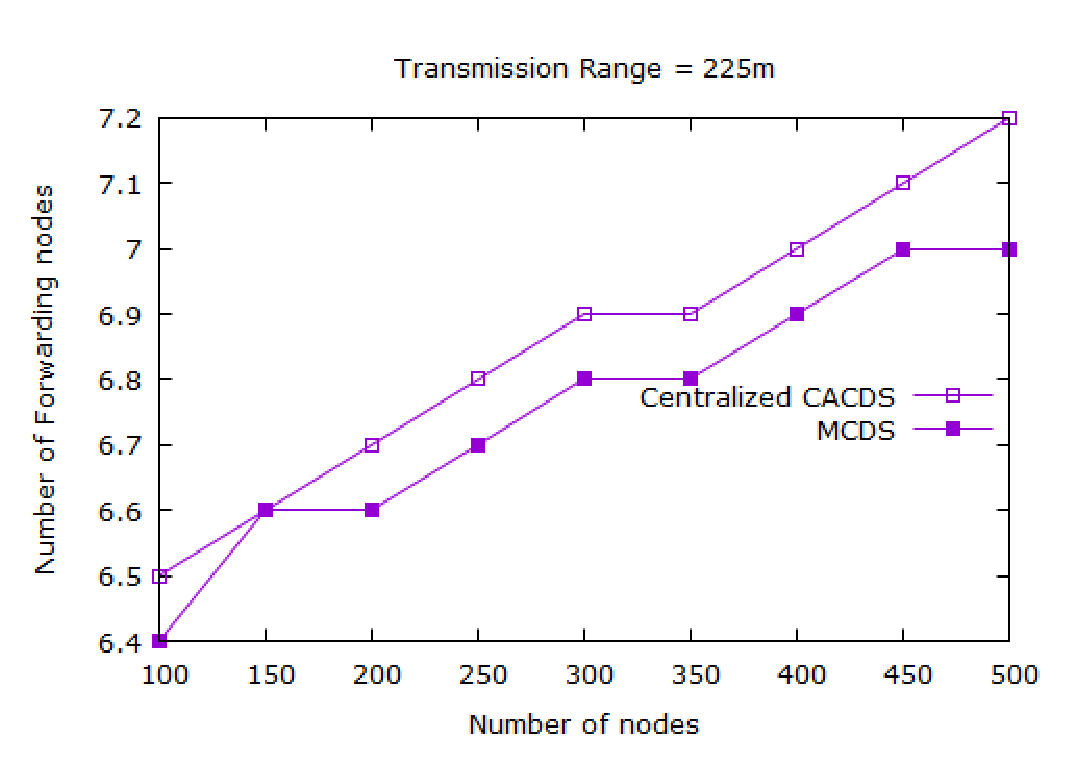
\includegraphics[width=90mm, height=57mm]{Figures/outf225c.eps}
    \caption{Performance of Centralized Algorithms for number of required transmissions by varying number of nodes}
    \label{outf225c}
    \end{figure}
    \begin{figure}[h]
    \centering
    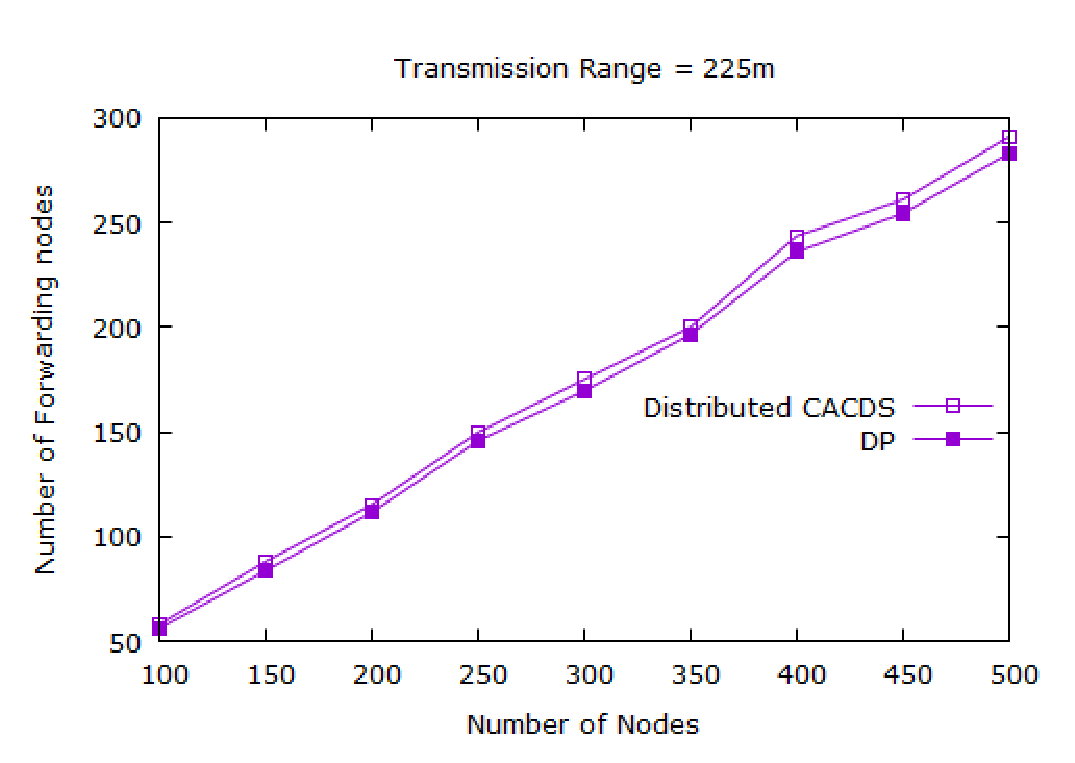
\includegraphics[width=90mm, height=57mm]{Figures/outf225d.eps}
    \caption{Performance of Distributed Algorithms for number of required transmissions by varying number of nodes}
    \label{outf225d}
\end{figure}

\subsection{Experimental Results regarding the Number of Contention}
\begin{figure}[h]
    \centering
    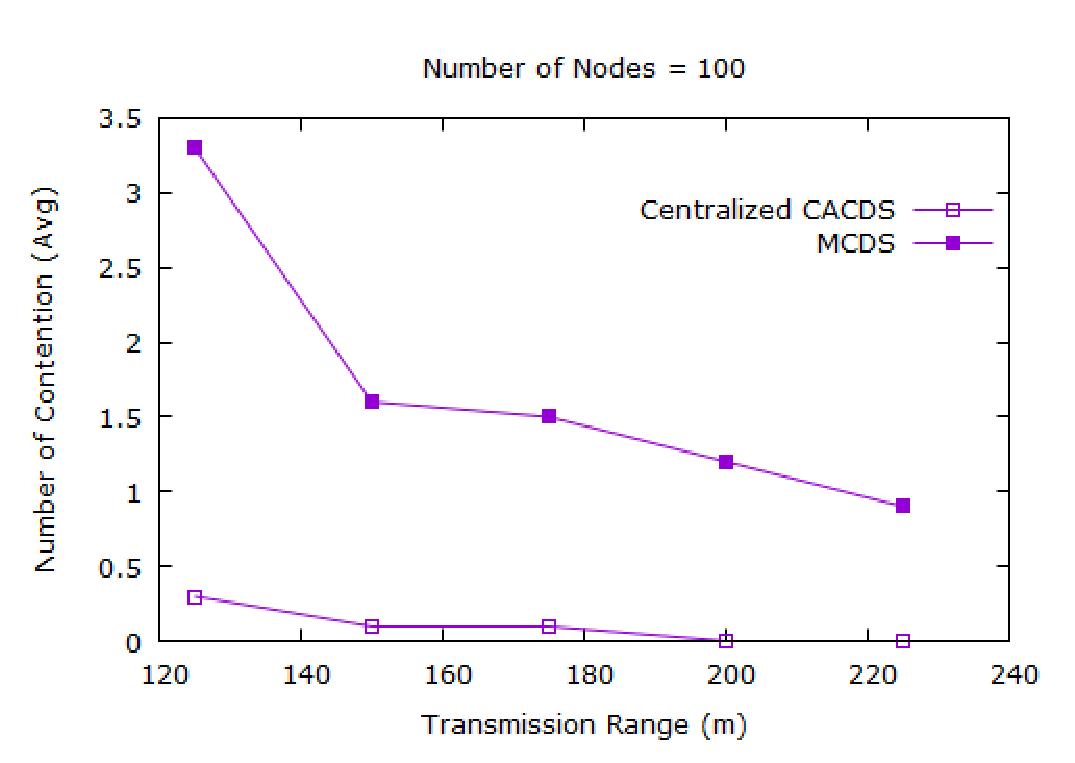
\includegraphics[width=90mm, height=57mm]{Figures/outc100c.eps}
    \caption{Performance comparison of Centralized Algorithms in term of contention varying transmission range}
    \label{outc100c}
    \end{figure}
    \begin{figure}[h]
    \centering
    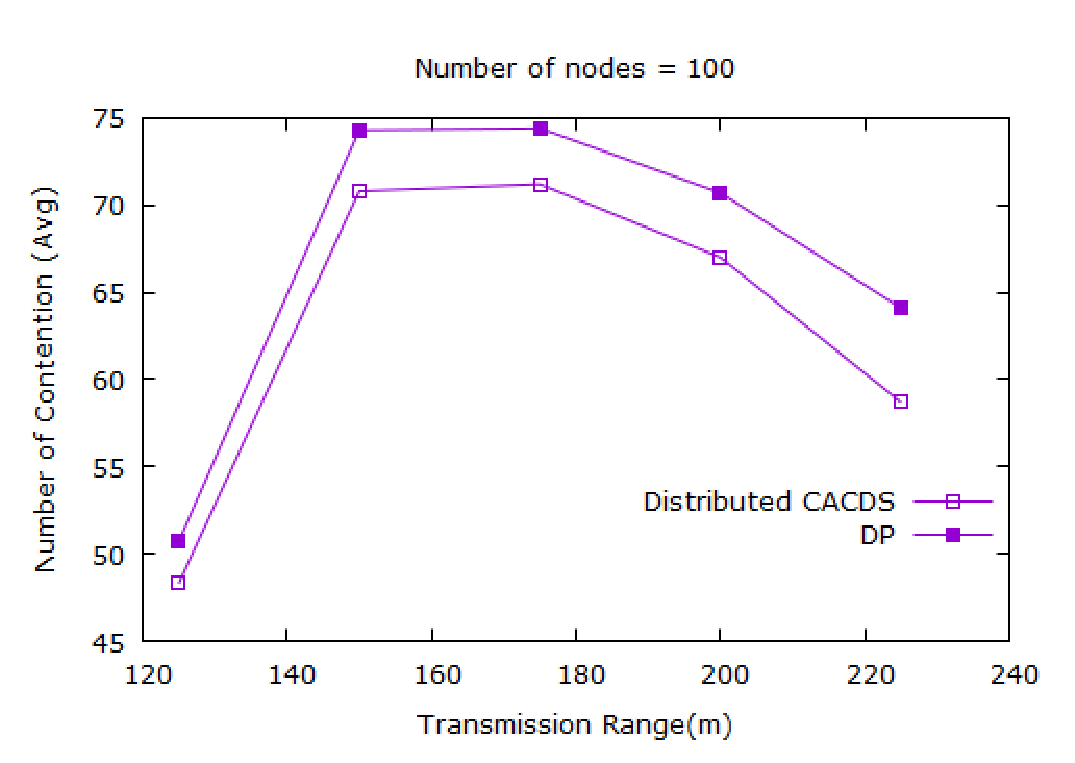
\includegraphics[width=90mm, height=57mm]{Figures/outc100d.eps}
    \caption{Performance comparison of Distributed Algorithms in term of contention varying transmission range}
    \label{outc100d}
\end{figure}

Figure \ref{outc100c} and Figure \ref{outc100d} present the state of contention occurrence for a sparse network with 100 nodes for both the centralized and distributed algorithms respectively. Figure \ref{outc100c} shows that the number of contention varies from 0.9 to 3.3 (in average) between the forwarding nodes in MCDS algorithm whereas it is minimized to 0-0.3 (in average) for Centralized CACDS. It is noticeable that for transmission range 225m, new algorithm generates totally contention free CDS. The distributed scenario is presented in Figure \ref{outc100d}. In distributed environment also, proposed method performs better than that of DP. It  avoids almost 4-9\% contention. In the scenario shown in Figure \ref{outc225c} and Figure \ref{outc225d} we vary number of nodes by keeping the transmission range set to 225m. Needless to say that, the new approaches also perform well.
\begin{figure}[h]
    \centering
    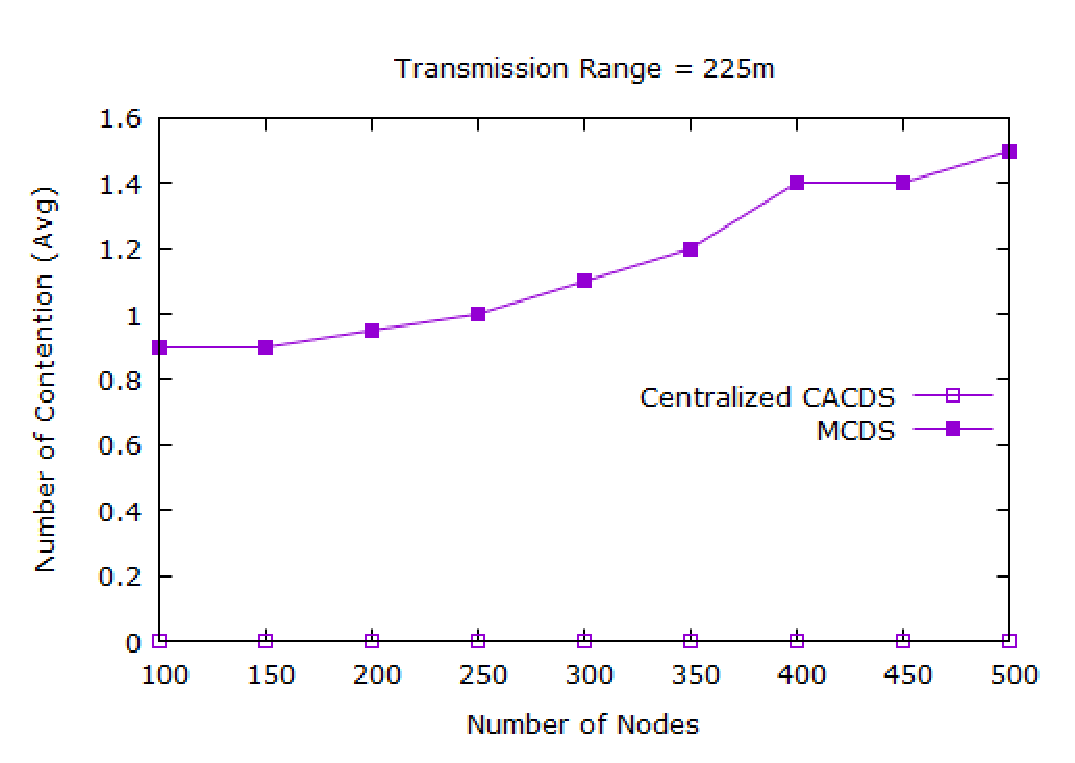
\includegraphics[width=90mm, height=57mm]{Figures/outc225c.eps}
    \caption{Performance comparison of Centralized Algorithms in term of contention varying number of nodes}
    \label{outc225c}
    \end{figure}
    \begin{figure}[h]
    \centering
    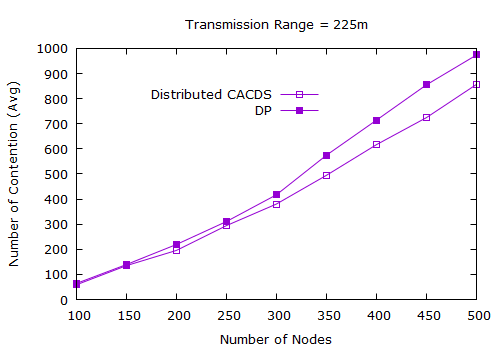
\includegraphics[width=90mm, height=57mm]{Figures/outc225d.png}
    \caption{Performance comparison of Distributed Algorithms in term of contention varying number of nodes}
    \label{outc225d}
\end{figure}

